\documentclass[intern]{cgMA}
\usepackage{titlesec}
\usepackage{graphicx}
\usepackage{float}
\usepackage{pdfpages}
\usepackage{array}
\usepackage{longtable}
\usepackage{booktabs}
\usepackage{svg}
\usepackage[
    backend=biber,
    style=numeric,
    sorting=none
]{biblatex}
\addbibresource{myBib.bib}

\usepackage{tocloft}
\usepackage{secdot}

\sectiondot{section}
\sectiondot{subsection}
\sectiondot{subsubsection}

\renewcommand{\cftsecaftersnum}{.}
\renewcommand{\cftsubsecaftersnum}{.}
\renewcommand{\cftsubsubsecaftersnum}{.}


\newenvironment{new_abstract}{
  \vspace*{\fill}
  \begin{center}%
    \bfseries\abstractname
  \end{center}}%
  {\vfill}


\graphicspath{ {./Images/} }

\setcounter{secnumdepth}{4}

\title{Untersuchung alternativer spielerbezogener Eingabemethoden in Videospielen am Beispiel eines prototypischen Horror-
Mystery-Spiels}
\author{Lea Olt}
\zweitgutachter{Katharina Krämer, M.Sc.}
\zweitgutachterInfo{(Institut für Computervisualistik, AG Computergraphik)}
\externLogo{7.46cm}{logos/ExternLogoPlaceholder}
\externName{DIN: NewTechnologies}

\begin{document}

   \maketitle  
\newpage
\thispagestyle{empty}
\quad 
\newpage

\begin{center}
  \textbf{\textit{Danksagung}}
  \end{center}
  \begin{center}
\textit{Test}
\end{center}
\newpage
\thispagestyle{empty}
\quad 
\newpage

%\section*{Zusammenfassung}
\begin{new_abstract}
Diese Arbeit behandelt die Untersuchung alternativer Eingabemethoden für Videospiele anhand eines Horror Mystery Prototypen. Der Fokus lag hierbei auf der zusätzlichen Komponente der gesichtsbasierten Eingabe durch Mimik und Blinzeln. 
\end{new_abstract}
\selectlanguage{english}
\begin{new_abstract}

\end{new_abstract}
\selectlanguage{ngerman}
\newpage

\thispagestyle{empty}
\quad 
\newpage

\tableofcontents
\newpage
\pagenumbering{arabic}
\section{Einleitung}

Ziel dieser Arbeit ist es,...
\section{Grundlagen}
Dieses Kapitel behandelt die technischen und theoretischen Grundlagen, auf denen der in dieser Arbeit entwickelte Prototyp aufbaut. Zunächst wird auf die
\subsection{Alternative Eingabemethoden}
Klassische Eingabemethoden wie Maus, Tastatur und Controller gehören zu den heutigen Standarts der Spieleindustrie. Sie sind leicht zugänglich, erfordern kaum zusätzlichen Aufwand und sind unabhängig von der Umgebung des Spielers. Die Interaktion erfolgt meist über das Betätigen von Tasten und Knöpfen, wodurch Bewegungen und Aktionen innerhalb der virtuellen Spielwelt ausgelöst werden. Obwohl es für die meisten Menschen heutzutage als natürliche Interaktion abgespeichert ist, bildet es die natürliche Verhaltens- und Bewegungsweise des Menschen nur abstrahiert ab. Die eigentliche körperliche Interaktion beschränkt sich dabei meist nur auf Hände, während körperliche Reaktionen, wie Mimik oder Gestik oft unberücksichtigt bleiben.
Bereits seit einigen Jahren wird versucht, den Spieler stärker in das Spielgeschehen einzubeziehen und natürlichere Formen der Interaktion zu ermöglichen. Bekannte Beispiele sind hierbei sie Nintendo Wii und die Microsoft Kinect. Beide Systeme ermöglichen eine körpergesteuerte Interaktion mit dem System. Mithilfe spezieller Sensorik werden reale Körperbewegungen Teil der Interaktion und ersetzen oder ergänzen herkömmliche Eingabemethoden. Allerdings setzen solche Systeme zusätzliche Hardware und Bewegungsraum voraus.\cite{wiiKinect}\cite{gilleade2005affective}.
\subsection{MediaPipe}
Für die Erfassung und Analyse des Gesichts des Spielers wird in dieser Arbeit MediaPipe verwendet. MediaPipe ist ein von Google entwickeltes Open-Source-Framework, welches verschiedene Verfahren zur Verarbeitung visueller Eingabedaten bereitstellt. Es bietet unter anderem Lösungen zur Gesten-, Hand-, und Gesichtserkennung. Für die vorliegende Arbeit ist insbesondere die Gesichtserkennung - genauer die Face landmark detection - relevant. Der Face Landmarker basiert dabei auf mehreren aufeinander aufbauenden Modellen. Zunächst wird mithilfe eines Face-Detection-Modells ein Gesicht im Eingabebild lokalisiert. Anschließend bestimmt ein Face-Mesh-Modell die Position von insgesamt 478 dreidimensionalen Face Landmarks. Darauf aufbauend kann ein weiteres Modell 52 Blendshape Scores berechnen, welche unterschiedliche Ausprägungen sichtbarer Gesichtsbewegungen repräsentieren \cite{google_mediapipe_face_landmarker}.\cite{emotionRecMediapipe}
\subsubsection{Face Landmarks}
Face Landmarks beschreiben charakteristische Punkte innerhalb eines erkannten Gesichts. Wie in Grafik X zu sehen werden 478 Punkte bestimmt, welche zusammen ein Face Mesh bilden und repräsentieren verschiedene Regionen im Gesicht. Die einzelnen Punkte werden durch dreidimensionale Koordinaten beschrieben.\cite{google_mediapipe_face_landmarker} Dabei stellen die Face Landmarks nur geometrische Informationen bereit und bieten selbst keine Interpretation des Gesichts. Durch das Analysieren der einzelnen Positionen und Abstände ausgewählter Punkte, können bestimmte Merkmale abgeleitet werden. Beispielsweise lässt sich anahand von Punkten entlang des Augenlids bestimmen, wie weit ein Auge geöffnet oder geschlossen ist. In dieser Arbeit bilden die Face Landmarks daher die Grundlage für die Erkennung von Blinzelbewegungen. Hierfür werden ausgewählte Landmark-Punkte im Bereich der Augen zur Berechnung der Eye Aspect Ratio (EAR) verwendet. Das zugrunde liegende Verfahren wird in Kapitel X näher erläutert.
\begin{figure}[H]
    \centering
    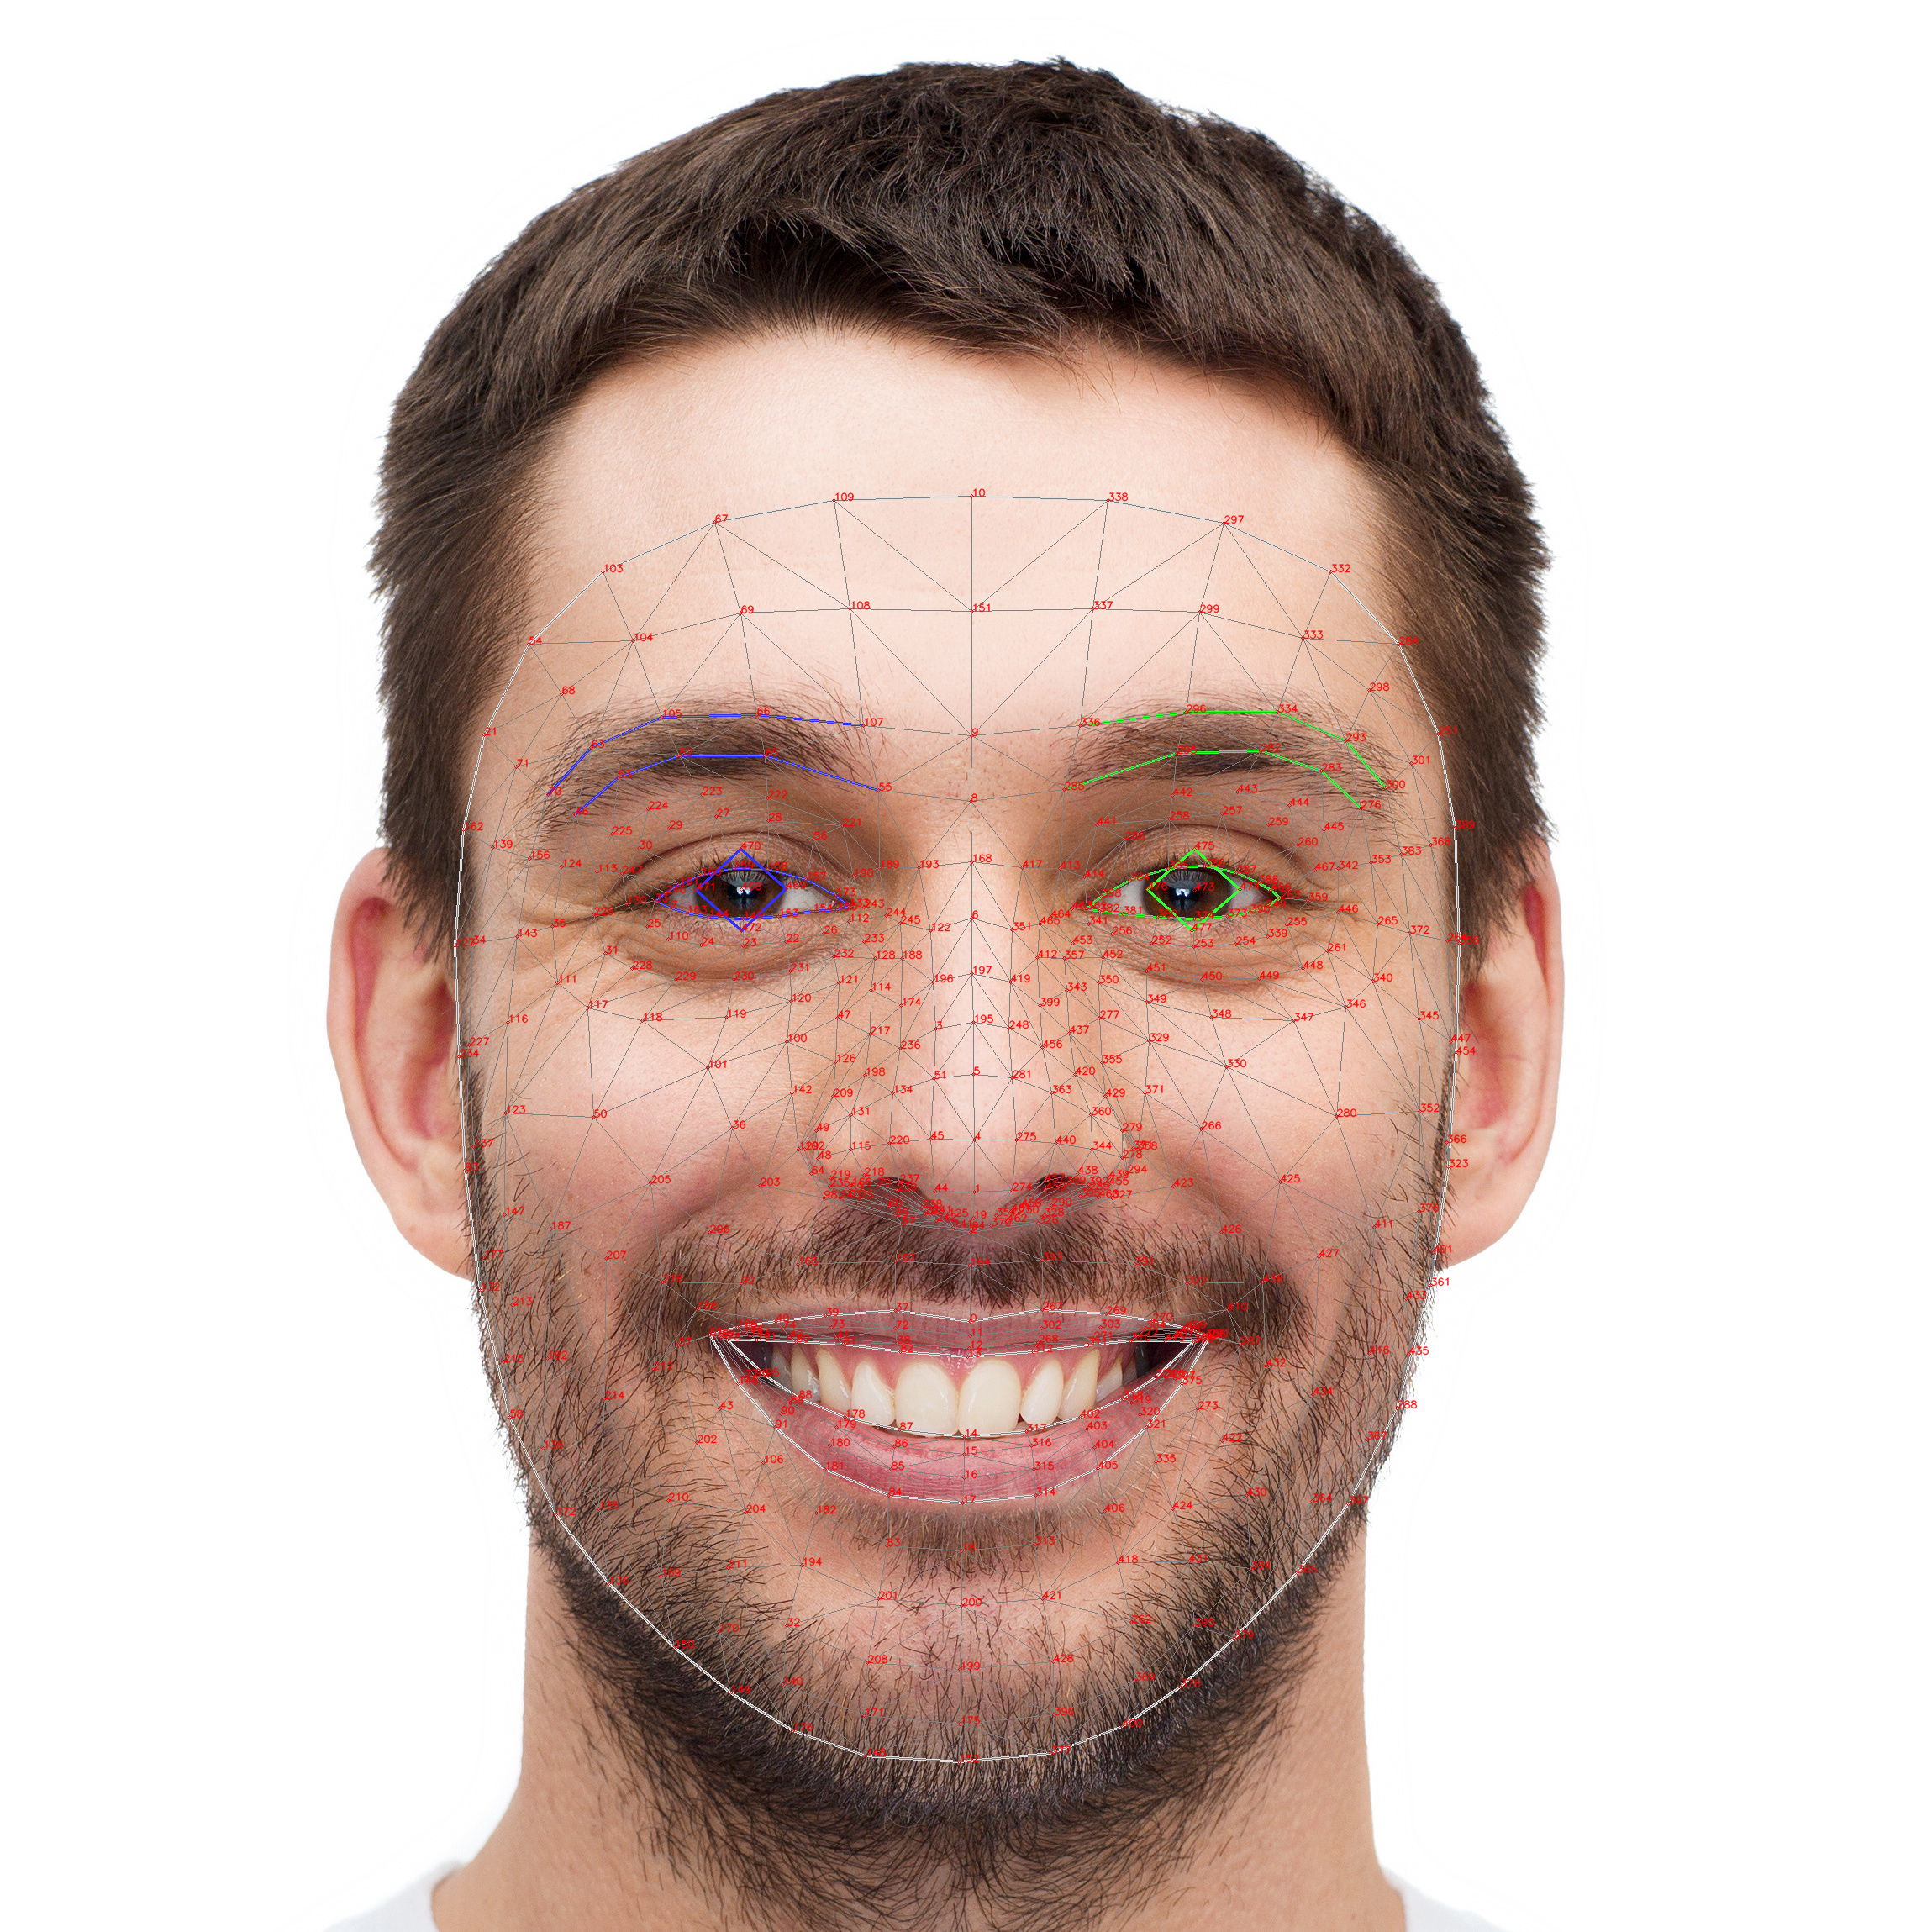
\includegraphics[width=0.5\textwidth]{Bilder/landmarks.png}
    \caption{Übersicht der vom MediaPipe ausgegebenen Face Landmarks.\cite{google_mediapipe_face_landmarker}}
    \label{fig:facs}
\end{figure}
\subsubsection{Blendshapes}
Blendshapes dienen zur Beschreibung einzelner Gesichtsbewegungen. Ausgangspunkt ist dabei ein neutrales Gesichtsmodell, von dem bestimmte Formen abgeleitet werden. Ein einzelner Blendshape repräsentiert jeweils eine konkrete Gesichtsbewegung, beispielsweise das Anheben einer Augenbraue oder das Heben eines Mundwinkels. Mediapipe stellt für die Gesichtsanalyse insgesamt 52 Blendshapes bereit, die verschiedene Bewegungen unter anderem in Bereich der Augenbrauen, Wange, Nase und Mund beschreiben. Die Werte liegen hierbei zwischen 0 und 1 und geben die geschätzte Intensität der jeweiligen Gesichtsverformung an. Einzelne Blendshapes besitzen dabei keine psychologische Bedeutung und stellen insbesondere keine direkte Emotion dar. Eine mögliche Interpretation bietet die Zuordnung der Blendshapes zu den Action Units des Facial Action Coding Systems (FACS), welches in Kapitel X näher erläutert wird.\cite{turrisi2026blendshape}
\subsection{Eye Aspect Ratio (EAR)}
Zur Blinzelerkennung wird in dieser Arbeit die Eye Aspect Ratio (EAR) eingesetzt. Der EAR-Wert bildet den geschätzten Öffnungsgrad des Auges ab. Der EAR-Wert wird aus sechs Landmarks pro Auge berechnet (zwei horizontale Eckppunkte, sowie zwei Paare vertikaler Punkte entlang des oberen und unteren Augenlids siehe Figur X). Dazu wird folgende Formel benutzt.
\begin{equation}
    \text{EAR} = \frac{\Vert p_2 - p_6 \Vert + \Vert p_3 - p_5 \Vert}{2 \cdot \Vert p_1 - p_4 \Vert}
\end{equation}
Ein Blinzeln kann erkannt werden, wenn der EAR-Wert unter einen definierten Schwellenwert fällt. Ein  zentrales Problem hierbei ist, dass die Werte stark zwischen unterschiedlichen Personen variieren. Grund dafür ist, dass jede Augenform und -größe individuell ist und durch verschiedene Kameraposition und -winkel die Augenform anders dargestellt werden kann. Ein fixer Schwellenwert liefert daher nicht für alle Nutzenden zuverlässige Ergebnisse. Aus diesem Grund wurde sich in der Arbeit für eine personenspezifische Kalibrierung des EAR-Schwellenwertes entschieden (siehe Kapitel X). \cite{earExplanation}
\begin{figure}[H]
    \centering
    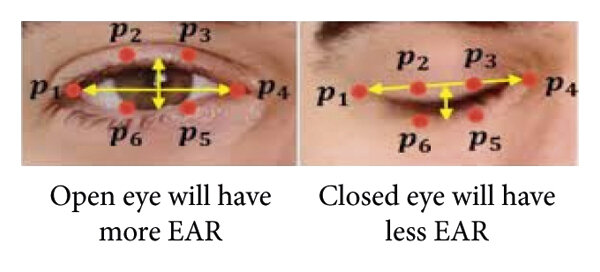
\includegraphics[width=0.5\textwidth]{Bilder/ear.jpg}
    \caption{Darstellung der EAR-Berechnung.\cite{earBasics}}
    \label{fig:facs}
\end{figure}
\subsection{Facial Action Coding System (FACS)}
Das Facial Action Coding System (FACS) dient der systematischen Beschreibung sichtbarer Gesichtsbewegungen. Hierzu werden mimische Veränderungen anhand sogenannter Action Units (AUs) codiert. Eine Action Unit beschreibt eine bestimmte beobachtbare Gesichtsbewegung und kann durch die Aktivität mehrerer Gesichtsmuskeln entstehen. Umgekehrt können einzelne Muskeln an verschiedenen Action Units beteiligt sein. Eine Übersicht ausgewählter Action Units und der jeweils beteiligten Gesichtsmuskulatur ist in Tabelle X dargestellt.\\
Für die Beschreibung emotionaler Gesichtsausdrücke wurde aufbauend auf FACS das Emotional Facial Action Coding System (EMFACS) entwickelt. Während FACS grundsätzlich sämtliche sichtbaren Gesichtsbewegungen codiert, konzentriert sich EMFACS auf diejenigen Action Units und Kombinationen von Action Units, die mit bestimmten emotionalen Gesichtsausdrücken in Verbindung gebracht werden.\cite{facsStimuli} Dabei kann ein emotionaler Gesichtsausdruck durch unterschiedliche Kombinationen von Action Units repräsentiert werden. Umgekehrt können einzelne Action Units Bestandteil verschiedener emotionaler Gesichtsausdrücke sein.\cite{turrisi2026blendshape}\cite{facialActionCodingReview}\\
So wird beispielsweise Freude unter anderem durch AU12 (Lip Corner Puller) oder durch die Kombination aus AU6 (Cheek Raiser) und AU12 beschrieben. Für Wut werden dagegen verschiedene mögliche Kombinationen angegeben, die beispielsweise AU4 (Brow Lowerer), AU5 (Upper Lid Raiser) und AU7 (Lid Tightener) enthalten können. Auch für Ekel, Angst, Traurigkeit und Überraschung werden unterschiedliche Kombinationen von Action Units beschrieben. Tabelle X zeigt eine Übersicht der Action-Unit-Kombinationen, die verschiedenen emotionalen Gesichtsausdrücken zugeordnet werden. Die dargestellten Zuordnungen basieren auf den von Ekman et al. beschriebenen Regeln. \cite{facsStimuli}\\
\begin{table}[H]
    \centering
    \footnotesize
    \setlength{\tabcolsep}{4pt}
    
    \caption{Zuordnung von Action Units (AUs) zu Emotionen nach dem FACS Investigators' Guide. A/B bedeutet, dass entweder A oder B auftreten kann.}
    \label{tab:facs-emotions}
    
    \begin{tabular}{p{2.2cm} p{7.5cm}}
        \toprule
        \textbf{Emotion} & \textbf{Action Units (AUs)} \\
        \midrule
        
        Anger &
        \begin{tabular}[t]{@{}l@{}}
        4+5+7+10+22+23+25/26 \\
        4+5+7+10+23+25/26 \\
        4+5+7+17+23/24 \\
        4+5+7+23/24 \\
        4+5/7 \\
        17+24
        \end{tabular}
        \\[0.5ex]
        
        \midrule
        
        Disgust &
        \begin{tabular}[t]{@{}l@{}}
        9/10+17 \\
        9/10+16+25/26 \\
        9/10
        \end{tabular}
        \\[0.5ex]
        
        \midrule
        
        Fear &
        \begin{tabular}[t]{@{}l@{}}
        1+2+4 \\
        1+2+4+5+20+25/26/27 \\
        1+2+4+5+25/26/27 \\
        1+2+4+5 \\
        1+2+5+25/26/27 \\
        5+20+25/26/27 \\
        5+20 \\
        20
        \end{tabular}
        \\[0.5ex]
        
        \midrule
        
        Happy &
        \begin{tabular}[t]{@{}l@{}}
        12 \\
        6+12
        \end{tabular}
        \\[0.5ex]
        
        \midrule
        
        Sadness &
        \begin{tabular}[t]{@{}l@{}}
        1+4 \\
        1+4+11/15 \\
        1+4+15+17 \\
        6+15 \\
        11+17 \\
        1
        \end{tabular}
        \\[0.5ex]
        
        \midrule
        
        Surprise &
        \begin{tabular}[t]{@{}l@{}}
        1+2+5+26/27 \\
        1+2+5 \\
        1+2+26/27 \\
        5+26/27
        \end{tabular}
        \\
        
        \bottomrule
    \end{tabular}
\end{table}

Diese Zuordnungen ermöglichen es, beobachtbare Gesichtsbewegungen anhand definierter Merkmale bestimmten Kategorien emotionaler Gesichtsausdrücke zuzuordnen. Dabei ist jedoch zwischen einem sichtbaren Gesichtsausdruck und dem tatsächlich empfundenen emotionalen Zustand einer Person zu unterscheiden. Das Auftreten einer bestimmten Kombination von Action Units bedeutet nicht zwangsläufig, dass die Person die damit assoziierte Emotion tatsächlich empfindet. In der Forschung wird unter anderem zwischen spontan auftretenden beziehungsweise „genuine“ und bewusst erzeugten beziehungsweise „posed“ Gesichtsausdrücken unterschieden. \cite{genuinePosedExpression}\\
Diese Unterscheidung ist für die vorliegende Arbeit von besonderer Bedeutung. Das entwickelte System verfolgt nicht das Ziel, den tatsächlichen inneren emotionalen Zustand des Spielers zuverlässig zu bestimmen. Stattdessen werden sichtbare Gesichtsbewegungen erfasst und zu definierten Gesichtsausdrücken zusammengefasst, die als zusätzliche Eingabe für das Spiel verwendet werden. Wird der Spieler beispielsweise dazu aufgefordert, einen wütenden Gesichtsausdruck zu zeigen, ist für die Spielmechanik entscheidend, ob die dafür definierten mimischen Merkmale erkannt werden, und nicht, ob der Spieler tatsächlich Wut empfindet.\\
Die durch FACS und EMFACS beschriebenen Zusammenhänge zwischen einzelnen
Gesichtsbewegungen und emotionalen Gesichtsausdrücken bilden damit eine
theoretische Grundlage für die Auswahl und Kombination der in dieser
Arbeit verwendeten MediaPipe-Blendshapes. Eine direkte Verbindung
zwischen beiden Repräsentationen wurde von Turrisi et al. untersucht.
Hierzu wurden die von MediaPipe bereitgestellten Blendshape Features
durch Experten systematisch den Action Units des FACS zugeordnet.
Die Ergebnisse zeigen eine hohe Übereinstimmung bei einem Großteil der
untersuchten Zuordnungen und verdeutlichen damit die Möglichkeit,
MediaPipe-Blendshapes als Grundlage für eine an FACS orientierte
Beschreibung von Gesichtsbewegungen zu verwenden
\cite{turrisi2026blendshape}.\\
Die konkrete Übertragung der für diese Arbeit relevanten Action Units
auf die verfügbaren MediaPipe-Blendshape-Scores sowie deren technische
Auswertung wird in Kapitel~5.4 näher erläutert.

\subsection{Affective Gameplay / Affective Computing}
Die vorliegende Arbeit ordnet sich in den Forschungsbereich des Affective Gameplay beziehungsweise Affective Computing in Videospielen ein. Dieser beschäftigt sich damit, wie emotionale Zustände von Spielenden erfasst und zur Anpassung oder Steuerung des Spielgeschehens genutzt werden können.\\
Eine für diese Arbeit zentrale Unterscheidung betrifft die Art, wie affektive Signale in das Spielgeschehen einfließen. Bei Biofeedback-Spielen kontrolliert die spielende Person ihren physiologischen oder mimischen Zustand bewusst und aktiv, um das Spielgeschehen zu beeinflussen. Bei affektiven Spielen hingegen fließen unkontrollierte, emotionale Reaktionen der spielenden Person in das Spiel ein, ohne dass diese versucht, ihren Zustand bewusst zu steuern.\cite{gilleade2005affective}\cite{Bersak2001IntelligentBU}\\
Diese Unterscheidung ist für die vorliegende Arbeit von Bedeutung, da die implementierte Spielmechanik (bewusstes Vermeiden von Blinzeln, aktives Zeigen aufgeforderter Emotionen) tendenziell dem aufgeforderten, biofeedback-artigen Pol zuzuordnen ist.
\section{Stand der Forschung}
Dieses Kapitel ordnet die vorliegende Arbeit in den bestehenden Forschungs- und Anwendungskontext ein. Zunächst werden konkrete Projekte und Spiele vorgestellt, die alternative, spielerbezogene Eingabemethoden umsetzen (3.1), gefolgt von einer vertieften Betrachtung von Affective-Gameplay- und Biofeedback-Ansätzen in Spielen (3.2). Abschließend wird die vorliegende Arbeit anhand der dargestellten Projekte und der in Kapitel 2 erarbeiteten Konzepte eingeordnet (3.3).
\subsection{Alternative spielerbezogene Eingaben in Videospielen}
Bereits die Nintendo Wii und die Microsoft Kinect zeigten, dass sich Spielende über Körperbewegung statt klassischer Tasteneingabe stärker in das Spielgeschehen einbeziehen lassen. Francese, Passero und Tortora \cite{wiiKinect} untersuchten bereits 2012 beide Systeme unter anderem hinsichtlich ihrer Usability sowie des dabei erzeugten Präsenz- und Immersionsgefühls und zeigten, dass körpergesteuerte Interaktion die wahrgenommene Immersion positiv beeinflussen kann, jedoch auf Kosten zusätzlicher Hardware und benötigten Bewegungsraums.\\
Neben körperbasierten Eingaben existieren weitere Ansätze, die spezifisch das Verhalten des Spielers vor dem Bildschirm einbeziehen. \textit{One Hand Clapping} nutzt die Stimme der spielenden Person als Ergänzung zur klassischen Steuerung. Dabei wird hier der Spielende explizit dazu aufgefordert Geräusche zu machen wohingegen bei dem Spiel \textit{Don't Scream} während des gesamten Spiels nicht geschrien werden darf auch wenn der Spielende sich erschreckt.\\
Bereits 2013 wurde an der Universität Regensburg ein Projekt durchgeführt, das die Blickrichtung der spielenden Person in ein Spiel einbezog. Sah die Person auf eine im Spiel vorhandene Fluchtmöglichkeit, verschwand diese. Gleiches galt für Verstecke. Derartige Projekte waren zum damaligen Zeitpunkt technisch noch mit hohem Aufwand und hohen Kosten verbunden, bezogen sich jedoch bereits meist auf echte, nicht aufgeforderte Emotionen bzw. Verhaltensweisen der spielenden Person.\cite{regensburg2013sophia} Andere frühe Projekte forderten Spielende hingegen explizit dazu auf, bestimmte Emotionen zu zeigen.\\
Ein besonders eng mit der vorliegenden Arbeit verwandtes Projekt ist Vigil (2025). Es ist ein Webcam-basiertes Horror-Spiel, in dem sich der Gegner, analog zu den Weeping Angels aus der britischen Fernsehserie Doctor Who, nur dann bewegt, wenn die spielende Person blinzelt oder wegschaut. Die Studie betont zudem, gestützt auf Flatla et al. (2011)\cite{calibrationFlatla}, die zentrale Bedeutung einer sorgfältig gestalteten Kalibrierung für die Nutzbarkeit blinzelbasierter Eingabesysteme, da eine misslungene oder unklare Kalibrierung die Interaktion mit dem System erheblich beeinträchtigen kann.\cite{vigilBlink}
\subsection{Affective Gameplay und Biofeedback in Spielen}
Nevermind (Flying Mollusk) gilt als eines der umfassendsten Beispiele eines vollständigen Biofeedback-Spiels: Über einen Herzfrequenzmesser wird der physiologische Erregungszustand der spielenden Person kontinuierlich erfasst; steigt die Anspannung, wird die Horror-Spielwelt bedrohlicher und schwerer zu bewältigen. Die spielende Person wird dadurch implizit dazu angehalten, den eigenen Erregungszustand aktiv zu regulieren.

APEX of Fear, ein VR-Horror-Spiel, verfolgt ein ähnliches Prinzip innerhalb einer immersiveren VR-Umgebung.

Ein frühes, grundlegendes Beispiel für ein Biofeedback-Spiel im engeren Sinne liefern Bersak et al. (2001) mit Relax-to-Win: Zwei Spielende treten mit animierten Drachen gegeneinander an, wobei die Geschwindigkeit des eigenen Drachens von der über den galvanischen Hautleitwert gemessenen Entspannung abhängt – wer sich am meisten entspannt, gewinnt. Interessant an diesem Beispiel ist, dass der Wettbewerbscharakter des Spiels dem eigentlichen Ziel (Entspannung) entgegenwirkte: Spielende wurden durch den Leistungsdruck tendenziell angespannter, mussten also lernen, ihre natürliche physiologische Reaktion aktiv zu überwinden, um erfolgreich zu sein.

Gilleade, Dix und Allanson (2005) unterscheiden auf dieser Grundlage zwischen Biofeedback-Spielen, bei denen die spielende Person ihren physiologischen Zustand bewusst kontrolliert, um das Spiel zu beeinflussen, und affektiven Spielen im engeren Sinne, bei denen unkontrollierte, teils der Person selbst nicht bewusste affektive Reaktionen erfasst werden. Relax-to-Win verdeutlicht dabei, dass die Grenze zwischen beiden Kategorien fließend sein kann: Zu Beginn reagieren Spielende meist unkontrolliert (affektiv), lernen im Spielverlauf jedoch zunehmend, ihre Reaktion bewusst zu steuern (Biofeedback).

Eine begleitende Studie zu Vigil (siehe Kapitel 3.1) greift genau diese Spannung explizit für die Blinzel-Mechanik auf: Blinzeln wird dort als Übergang von einem unwillkürlichen, reflexartigen Vorgang hin zu einer bewusst gesteuerten Spielmechanik beschrieben – die Studie spricht von "voluntary control of involuntary inputs". Sie stützt sich dabei unter anderem auf den Begriff des "affective feedback" nach Dekker und Champion (2007), wonach emotionale Reaktionen nicht nur Ergebnis, sondern aktiver Bestandteil der Steuerungsschleife sind, sowie auf Befunde, nach denen insbesondere die Blink-Amplitude (nicht die reine Blinzelrate) mit affektiver Erregung in Verbindung steht [Vigil-Designing-Fear-Paper, 2025/2026]. Diese Einordnung liegt konzeptuell sehr nah an der in Kapitel 2.4 und 2.5 dargestellten Unterscheidung zwischen aufgeforderten und genuinen affektiven Reaktionen und wird in Kapitel 3.3 wieder aufgegriffen.

Diese Projekte zeigen übereinstimmend, dass sich physiologische und affektive Signale gezielt zur Verstärkung von Horroratmosphäre einsetzen lassen, unterscheiden sich jedoch darin, ob die zugrundeliegenden affektiven Zustände genuin (Nevermind, Regensburg-Studie) oder aufgefordert (Don't Scream, Vigil, Teile dieser Arbeit) erzeugt werden.
\subsection{Einordnung der eigenen Arbeit}
Die dargestellten Arbeiten zeigen, dass die grundlegende Idee, Spielende über ihr reales Verhalten oder physiologische Signale in das Spielgeschehen einzubeziehen, bereits seit längerer Zeit Gegenstand der Forschung ist. Frühere Ansätze waren dabei teilweise auf spezialisierte und kostenintensive Hardware angewiesen. Durch heutige Verfahren der kamerabasierten Gesichtsanalyse ergeben sich hingegen Möglichkeiten, vergleichbare Interaktionskonzepte mit handelsüblicher Hardware umzusetzen. Die vorliegende Arbeit greift diesen Ansatz auf und untersucht mit MediaPipe eine ausschließlich webcam-basierte Möglichkeit zur Erfassung spielerbezogener Eingaben.\\
Im Unterschied zu klassischen Affective Games steht dabei nicht die Erfassung spontan auftretender emotionaler Zustände im Vordergrund. Stattdessen werden die Spielenden gezielt dazu aufgefordert, bestimmte Gesichtsausdrücke zu zeigen oder körperliche Reaktionen wie das Blinzeln bewusst zu kontrollieren. Damit weisen die untersuchten Eingabemethoden sowohl Merkmale bewusst gesteuerter Eingaben als auch Parallelen zu biofeedback-basierten Spielmechaniken auf. Eine eindeutige Zuordnung zu den zuvor beschriebenen Kategorien ist daher nur eingeschränkt möglich.\\
Während verwandte Arbeiten häufig einzelne Signale oder Interaktionsformen betrachten, kombiniert der entwickelte Prototyp Blinzeln und mimische Gesichtsausdrücke innerhalb eines Horror-Mystery-Spiels. Darüber hinaus werden eine personenspezifische Kalibrierung sowie visuelles Feedback als Bestandteile der Interaktion untersucht. Dadurch soll insbesondere betrachtet werden, welchen Mehrwert diese spielerbezogenen Eingabemethoden gegenüber einer konventionellen Steuerung bieten.
\section{Konzept}
In den folgenden Abschnitten wird ein Überblick über die Konzeption des in dieser Arbeit entwickelten Prototypen gegeben. Eine genaue technische umsetzung folgt in Kapitel 5.
\subsection{Zielsetzung und Anforderungen des Prototypen}
Ziel des Prototypen ist es, alternative spielerbezogene Eingabemethoden in einem konkreten Spielkontext zu untersuchen. Im Gegensatz zu einer klassischen Steuerung soll dabei das Verhalten der spielenden Person vor dem Bildschirm als Eingabe für das Spielgeschehen genutzt werden. Der Prototyp dient damit als experimentelle Grundlage, für die Frage, wie sich solche Eingabemethoden in bestehende Spielmechaniken integrieren lassen und welchen Einfluss sie auf das Spielerlebnis haben.\\
Für die Umsetzung wurde ein Horror-Mystery-Spiel gewählt. Das Genre bietet einen geeigneten Rahmen, um ungewöhnliche Eingabemethoden wie das bewusste Kontrollieren des Blinzelns oder das Zeigen bestimmter Gesichtsausdrücke in bedrohliche und unerwartete Spielsituationen einzubetten.\\
Eine weitere Anforderung besteht darin, dass für die Nutzung des Prototyps keine spezielle zusätzliche Hardware vorausgesetzt werden soll. Die Gesichtserfassung soll daher ausschließlich über eine handelsübliche Webcam passieren. Gleichzeitig musste berücksichtigt werden, dass Personen unterschiedliche Gesichtsmerkmale aufweisen. Aus diesem Grund wurde bereits bei der Konzeption eine personenspezifische Kalibrierung vorgesehen.\\
Darüber hinaus soll der Prototyp einen Vergleich mit einer konventionellen Eingabemethode ermöglichen. Die entwickelten Mechaniken wurden daher so konzipiert, dass sie auch nur mit Maus und Tastatur genutzt werden können. Dadurch kann im Rahmen der späteren Evaluation untersucht werden, wie die alternativen Eingabemethoden im Vergleich zu einer konventionellen Steuerung wahrgenommen werden.\\
Die folgenden Abschnitte beschreiben das Spielkonzept im Detail, die gewählten Eingabemethoden, die Kalibrierung sowie die Gestaltung der Spielmechaniken, die zur Untersuchung der Forschungsfrage eingesetzt werden.
\subsection{Spielkonzept}
Der entwickelte Prototyp ist ein Singleplayer-Spiel und spielt in einem Hotel. Der Spieler schlüpft in die Rolle eines Hotelangestellten, der in seiner Schicht verschiedene Aufträge abarbeiten muss. Die zentrale Aufgabe besteht darin, verschiedene Gegenstände zu bestimmten Hotelzimmern zu bringen. Hinter diesem zunächst einfachen Arbeitsablauf verbirgt sich jedoch mehr. Sowohl die Hotelgäste, welche manchmal einfach durch das Hotel laufen, als auch die zu liefernden Gegenstände besitzen Eigenschaften, die von einem gewöhnlichen Hotelbetrieb abweichen und den Spieler zur Interaktion mit den alternativen Eingabemethoden auffordern.\\
Der grundlegende Spielablauf basiert auf einem wiederkehrenden \textit{Delivery-System}. Zu Beginn eines Auftrags erhält der Spieler Informationen darüber, welcher Gegenstand zu welchem Hotelzimmer gebracht werden muss. Einige Gegenstände erfordern vor der Auslieferung eine zusätzliche Interaktion. Diese ist an bestimmte Gesichtsausdrücke oder an das Blinzeln gekoppelt. Erst nachdem die jeweilige Bedingung erfüllt wurde, können die Gegenstände erfolgreich abgeliefert werden. Nach erfolgreicher Auslieferung wird der nächste Auftrag freigeschaltet und dem Spieler präsentiert.\\
Neben den eigentlichen Lieferaufträgen begegnet der Spieler verschiedenen Hotelgästen beziehungsweise Gegnern, die ebenfalls auf sein Verhalten reagieren. Abhängig vom jeweiligen Gegnertyp können diese dem Spieler freundlich oder feindlich gesinnt sein und unterschiedliche Reaktionen erfordern.\\
Der zugrunde liegende Game Loop ist bewusst einfach gehalten. Das Abholen und Ausliefern der Gegenstände bildet lediglich den Rahmen, innerhalb dessen die eigentlichen Herausforderungen auftreten. Diese entstehen einerseits durch die besonderen Anforderungen der Gegenstände und andererseits durch Begegnungen mit den Hotelgästen während der Auslieferung. Die zunächst einfache und wiederkehrende Aufgabe wird dadurch immer wieder durch ungewöhnliche Situationen unterbrochen und erschwert.\\
Das Spiel endet entweder dadurch, dass der Spieler alle Aufträge erfolgreich abgeschlossen hat oder dadurch, das die Lebenspunkte des Spielers vollständig aufgebraucht sind. Lebenspunkte kann der Spieler insbesondere durch die Begegnung mit feindlich gesinnten Hotelgästen verlieren. Um die Fortbewegung und die Orientierung innerhalb des Spielgeschehens zu unterstützen wurde eine schnellere Fortbewegung mittels begrenzeter Ausdauer und eine Minimap hinzugefügt. Die Minimap dinent der orientierung innerhalb des Hotels und zeigt dem Spieler den Weg zum näcshten Auftragsziel an.\\
Darüber hianus kannd er Spieler im Laufe des Spielgeschehens Hilfsgegenstände erhalten. So kann beispielsweise durch eine erfolgreiche Interaktion mit einem Hotelgast eine Taschenlampe als Geschenk erhalten werden, die anschließend die Orientierung in dunklen Bereichen des Hotels erleichtert.
\subsection{Konzeption der spielerbezogenen Eingabemethoden}
\subsubsection{Blinzeln und Augenzustand}
Eine der zentralen spielerbezogenen Eingabemethoden des Prototyps ist die bewusste Kontrolle des Blinzelns. Dabei werden sowohl das Blinzeln selbst als auch das gezielte Offen- oder Geschlossenhalten der Augen als Eingabe verwendet. Ziel ist es, einen normalerweise automatischen Prozess des Körpers in eine bewusst kontrollierte Spielmechanik zu überführen.\\
Die Eingabe wird dabei in unterschiedlichen Situationen eingesetzt. Bei bestimmten Gegnern kann ein Blinzeln beispielsweise eine unmittelbare Reaktion auslösen, während andere Situationen erfordern, die Augen für einen bestimmten Zeitraum offen oder geschlossen zu halten. Dadurch kann die Eingabe in verschiedenen Kontexten spielerisch eingesetzt werden.
\subsubsection{Gesichtsausdrücke}
Als weitere spielerbezogene Eingabemethode werden bewusst erzeugte Gesichtsausdrücke verwendet. Für den Prototyp wurden die vier Ausdrücke Freude, Wut, Trauer und Überraschung ausgewählt. Im Gegensatz zu einer Erkennung des tatsächlichen emotionalen Zustands besteht das Ziel dabei nicht darin, Rückschlüsse auf die gegenwärtig empfundene Emotion des Spielers zu ziehen. Stattdessen werden die Gesichtsausdrücke bewusst als Eingabe eingesetzt und müssen in entsprechenden Spielsituationen gezielt erzeugt werden.\\
Die verschiedenen Gesichtsausdrücke können dabei unterschiedliche Reaktionen innerhalb der Spielwelt auslösen und werden als zusätzliche Eingabemöglichkeit neben der klassischen Steuerung eingesetzt. Da sich die Ausprägung der Mimik zwischen verschiedenen Personen unterscheiden kann, wurde bei der Konzeption berücksichtigt, dass die Erkennung an den jeweiligen Spieler angepasst werden muss. Die dafür vorgesehene personenspezifische Kalibrierung wird in Kapitel 4.X näher beschrieben.
\subsection{Integration in die Spielmechanik}
Bei der Zuordnung der spielerbezogenen Eingabemethoden zu konkreten Spielsituationen wurden drei unterschiedliche Kontexte gebildet. Zum einen die gegenstandsbezogenen Mechaniken, Interaktion mit Hotelgästen und zum anderen Umgebungsinteraktionen innerhalb der Spielwelt. Dabei wurde darauf geachtet, einen inhaltlichen Zusammenhang zwischen der geforderten Eingabe und ihrer Auswirkung zu schaffen. Somit sollen die Eingaben nicht lediglich als alternativer Auslöser fungieren sondern logisch in die die Spielsituation eingebunden werden.
\subsubsection{Liefer-Gegenstände}
Ein Teil der spielerbezogenen Eingabemethoden wird direkt mit den auszuliefernden Gegenständen verbunden. Bestimmte Gegenstände können nicht unmittelbar ausgeliefert werden, sondern müssen zuvor durch eine entsprechende Eingabe vorbereitet werden. Tabelle~\ref{tab:gegenstaende} gibt einen Überblick über die verschiedenen Gegenstände und die damit verbundenen Eingaben.
\begin{table}[H]
    \centering
    \caption{Übersicht der Gegenstände und der zugehörigen spielerbezogenen Eingaben}
    \label{tab:gegenstaende}
    \begin{tabularx}{\textwidth}{l X X}
        \hline
        \textbf{Gegenstand} & \textbf{Interaktion} & \textbf{Geforderte Eingabe} \\
        \hline

        Essen &
        Muss vor der Auslieferung auf die erforderliche Temperatur erhitzt werden. &
        Wütender Gesichtsausdruck \\

        Kerze &
        Der Zustand der Kerze wird durch das Blinzeln des Spielers beeinflusst. &
        Blinzeln \\

        Pflanze &
        Benötigt Licht, wobei eine zu starke Einwirkung vermieden werden muss. &
        Lächeln \\
        
        \hline
    \end{tabularx}
\end{table}
Bei der Zuordnung der Eingaben wurde teilweise ein inhaltlicher Zusammenhang zwischen dem jeweiligen Gesichtsausdruck und der Reaktion des Gegenstands hergestellt. So wird Wut als „hitzige“ Emotion mit dem Erhitzen der Mahlzeit verbunden. Das Lächeln wird bei der Pflanze hingegen mit Sonnenlicht assoziiert. Dabei muss der Spieler die Intensität der Interaktion kontrollieren, da eine zu starke Einwirkung einen negativen Effekt auf die Pflanze hat. Die Kerzenmechanik basiert dagegen nicht auf einer vergleichbaren symbolischen Zuordnung, sondern nutzt das Blinzeln unmittelbar als spielerische Eingabe.
\subsubsection{Hotelgäste / Gegner}
Neben den auszuliefernden Gegenständen bilden die verschiedenen Hotelgäste einen weiteren Anwendungsbereich der spielerbezogenen Eingabemethoden. Die Gäste unterscheiden sich in ihrem Verhalten und stellen unterschiedliche Anforderungen an den Spieler. Während einige eine unmittelbare Bedrohung darstellen, dienen andere eher als Hindernis oder lösen kurze Interaktionen aus.\\
Auch bei der Konzeption der Gäste wurde versucht, die geforderte Eingabe möglichst sinnvoll mit ihrem Verhalten oder der jeweiligen Situation zu verbinden. Dadurch sollen die Gesichtseingaben nicht lediglich eine klassische Tasteneingabe ersetzen, sondern Bestandteil der jeweiligen Begegnung sein. 
Tabelle~\ref{tab:gaeste_gegner} gibt einen Überblick über die konzipierten Gäste und die zugehörigen Eingaben. 
\begin{table}[H]
    \centering
    \caption{Übersicht der Gäste und Gegner sowie der zugehörigen spielerbezogenen Eingaben}
    \label{tab:gaeste_gegner}
    \begin{tabularx}{\textwidth}{l X X}
        \hline
        \textbf{Gast/Gegner} & \textbf{Verhalten und Konzept} & \textbf{Geforderte Eingabe} \\
        \hline

        BlinkEnemy &
        Von den Weeping Angels aus \textit{Doctor Who} \cite{doctorwhoWeepingAngels} inspirierter Gegner, der sich dem Spieler nähert, sobald er nicht beobachtet wird. &
        Nicht blinzeln / Blickkontakt halten \\

        SmileSwarm &
        Gruppe lächelnder Gegner, an deren Verhalten sich der Spieler anpassen muss, um nicht aufzufallen. &
        Lächeln \\

        CuteFluffyEnemy &
        Kleine Gegner, die dem Spieler keinen direkten Schaden zufügen, ihn jedoch durch das Blockieren seines Weges behindern. &
        Wütender Gesichtsausdruck \\

        Geschenk-Gast &
        Überreicht dem Spieler ein Geschenk und erwartet zunächst eine überraschte und anschließend eine erfreute Reaktion. &
        Überraschung, anschließend Freude \\

        GambleGuest &
        Fordert den Spieler zu einem Glücksspiel heraus, bei dem der Spieler am Ende die Augen schließen muss. &
        Augen schließen \\

        NoiseGuest &
        Reagiert auf Geräusche des Spielers und bewegt sich in Richtung der Geräuschquelle. &
        Geräusche vermeiden \\
        \hline
    \end{tabularx}
\end{table}
Bei einigen Gästen ergibt sich die geforderte Eingabe unmittelbar aus der jeweiligen Situation. Der Geschenk-Gast erwartet zunächst eine überraschte Reaktion auf das präsentierte Geschenk und anschließend Freude über dessen Erhalt. Beim SmileSwarm wird das Lächeln hingegen als Anpassung an das Verhalten der Gruppe eingesetzt: Der Spieler muss ebenfalls lächeln, um innerhalb der Gruppe nicht aufzufallen. Der BlinkEnemy ist konzeptionell durch die Weeping Angels aus Doctor Who\cite{doctorwhoWeepingAngels} inspiriert. Solange der Spieler den Gegner beobachtet, bleibt dieser stehen. Wird der Blickkontakt durch Wegschauen oder Blinzeln unterbrochen, kann sich der Gegner dem Spieler nähern. Das Blinzeln des Spielers wird dadurch selbst zu einem Risiko.
\subsubsection{Weitere Interaktionen}
Neben den Gegenständen und Hotelgästen werden die Gesichtseingaben auch für weitere Interaktionen innerhalb des Hotels verwendet. Dazu gehören unter anderem der Aufzug sowie verschiedene Zugangskontrollen.\\
Der Aufzug wird nicht ausschließlich über eine klassische Tasteninteraktion gesteuert, sondern bezieht die Mimik des Spielers mit ein. Ein trauriger Gesichtsausdruck wird dabei mit Tränen verbunden und für die Steuerung des Aufzugs verwendet. Dadurch wird auch die Fortbewegung innerhalb des Hotels mit einer der alternativen Eingabemethoden verknüpft.\\
Zusätzlich befinden sich an bestimmten Stellen des Hotels Zugangskontrollen, die eine bestimmte Eingabe vom Spieler verlangen. Der Spieler muss dafür vor dem jeweiligen Scanner beispielsweise einen geforderten Gesichtsausdruck zeigen oder für eine bestimmte Zeit den Blickkontakt halten. Erst nach erfolgreicher Erfüllung der Bedingung wird der entsprechende Zugang freigegeben.
\subsection{Kalibrierung}
Ein zentraler Bestandteil des Eingabekonzepts stellt die personenspezifische Kalibrierung dar. So wie in Kapitel XXX beschrieben die Größe und Form der Augen zwischen Personen sehr unterschiedlich sein kann, unterscheiden sich auch die Stärke und Art der Gesichtsausdrücke. Deswegen wurde vorgesehen, die Erkennung an jede Person individuell abzustimmen.\\
Als erster Schritt der Kalibrierung steht die Erfassung der Augen um den neutralen Augenöffnungswert der Person zu identifizieren. Danach wird zunächst die neutrale Mimik des Spielers erfasst und folgend nacheinander die einzelnen relevanten Gesichtsausdrücke, Freude, Wut, Trauer und Überraschung. Die dabei erfassten Werte dienen hierbei als persönliche Referenz relativ zum individuellen neutralen Gesichtsausdruck. Nach den jeweiligen Kalibrierungsetappen hat der Spieler immer die Möglichkeit die aktuelle Kalibrierung zu wiederholen. Abschließend wird der Spieler dazu aufgefordert die erkannten Gesichtszüge zu testen und gegebenenfalls erneut zu kalibrieren. \\
%Selbst geschrieben
Neben der reinen Kalibrierung spielte auch die Gestaltung eine Rolle. Flatla et al. \cite{flatla2011calibration} zeigen in ihrer Arbeit, dass klassische Kalibrierung oft als monoton und wenig unterhaltsam wahrgenommen werden. Deswegen schlagen sie vor, die Kalibrierung spielerisch besser zu verknüpfen. Dabei soll die eigentliche Kernaufgabe der Kalibrierung erhalten bleiben, aber die Darstellung beispielsweise durch ein thematisches Setting oder Fortschrittsbalken spielerischer gestaltet werden.\cite{flatla2011calibration}\\
Dieser Ansatz wurde bei der Gestaltung des Prototyps mit einbezogen. Zunächst wurde eine rein technisch und vom Spielgeschehen abgekapselte Kalibrierung umgesetzt. Danach wurde die Kalibrierung erst mit dem Spielgeschehen mit eingebunden. Der Spieler führt die Kalibrierung im Zuge einer Mitarbeiterregistierung aus. Dabei befindet sich der Spieler in einem Büro, in dem er dazu aufgefordert wird zur Registrierung bestimmte Gesichtsausdrücke zu machen.
\subsection{Feedbackkonzept}
%Eine besondere Rolle spielt dabei das Feedback für die Blinzelerkennung. Wird ein Blinzeln erkannt, schließen sich kurzzeitig virtuelle Augenlider über dem sichtbaren Spielbereich. Dadurch wird die erkannte Eingabe unmittelbar visuell an den Spieler zurückgegeben. Gleichzeitig verstärkt die Darstellung die Verbindung zwischen dem realen Blinzeln des Spielers und dem Zustand der Spielfigur, da sich deren Sicht entsprechend verändert.
Da die spielerbezogenen Eingaben nicht über physische Tasten erfolgen, ist für den Spieler nicht immer ersichtlich, welche Eingabe von dem System erkannt wurde. Aus diesem Grund wurden verschiedene Feedbackmechanismen eingebaut, die dem Spieler eine direkte Rückmeldung über die erkannte Eingabe gibt und gegebenenfalls auch zeigt, welche Auswirkung diese Eingabe in der Spielwelt hat. \\
Wird ein Blinzeln erkannt, schließen sich kurzzeitig virtuelle Augenlider über den sichtbaren Spielbereich (siehe Foto) Somit wird dem Spieler direkt visuell eine Rückmeldung gegeben, dass sein Blinzeln von dem System registriert wurde. Auch für die Erkennung der Gesichtsausdrücke wurde ein dauerhaftes visuelles Feedback vorgesehen. Eine Anzeige im sichtbaren Feld des Spielers, gibt ihm während des Spiels an, welcher Gesichtsausdruck aktuell erkannt wird.(FOTO) Neben dem dauerhaften Feedback hat der Spieler die Möglichkeit, sich zusätzlich seine aktuellen Eingabewerte grafisch anzeigen zu lassen. Diese Visualisierung zeigt dem Spieler sowohl seinen aktuellen Augenwert als auch die Stärke des erkannten Gesichtsausdrucks inklusive dem personenspezifischen Schwellenwert.\\
Darüber hinaus wurde für die verschiedenen Aufgaben, die der Spieler im Laufe des Spielgeschehens durch Gesichtseingaben bewältigen muss immer eine Form des direkten Feedbacks eingebaut. Beim Erhitzen des Essens wird beispielsweise durch einen Fortschrittsbalken dem Spieler unmittelbar angezeigt, wie sich sein Gesichtsausdruck auf den Gegenstand auswirkt. Gleiches verhält sich bei der Pflanze und bei dem Aufzug. Die Veränderung der Anzeige macht dadurch sichtbar, ob die gewählte Eingabe die gewünschte Wirkung erzielt. Bei anderen Mechaniken wie beispielsweise der Kerze wird durch visuelle Veränderung der Spielwelt dem Spieler gezeigt, dass seine Eingabe eine Wirkung hatte. So erlischt die Kerze, sobald der Spieler blinzelt. Ähnlich verhält es sich bei Zugangskontrollen oder Hotelgästen, die dem Spieler entweder durch visuelle Veränderung oder durch ein akustisches Signal vermitteln, ob eine geforderte Eingabe erfolgreich ausgeführt wurde.
\begin{figure}[H]
    \centering
    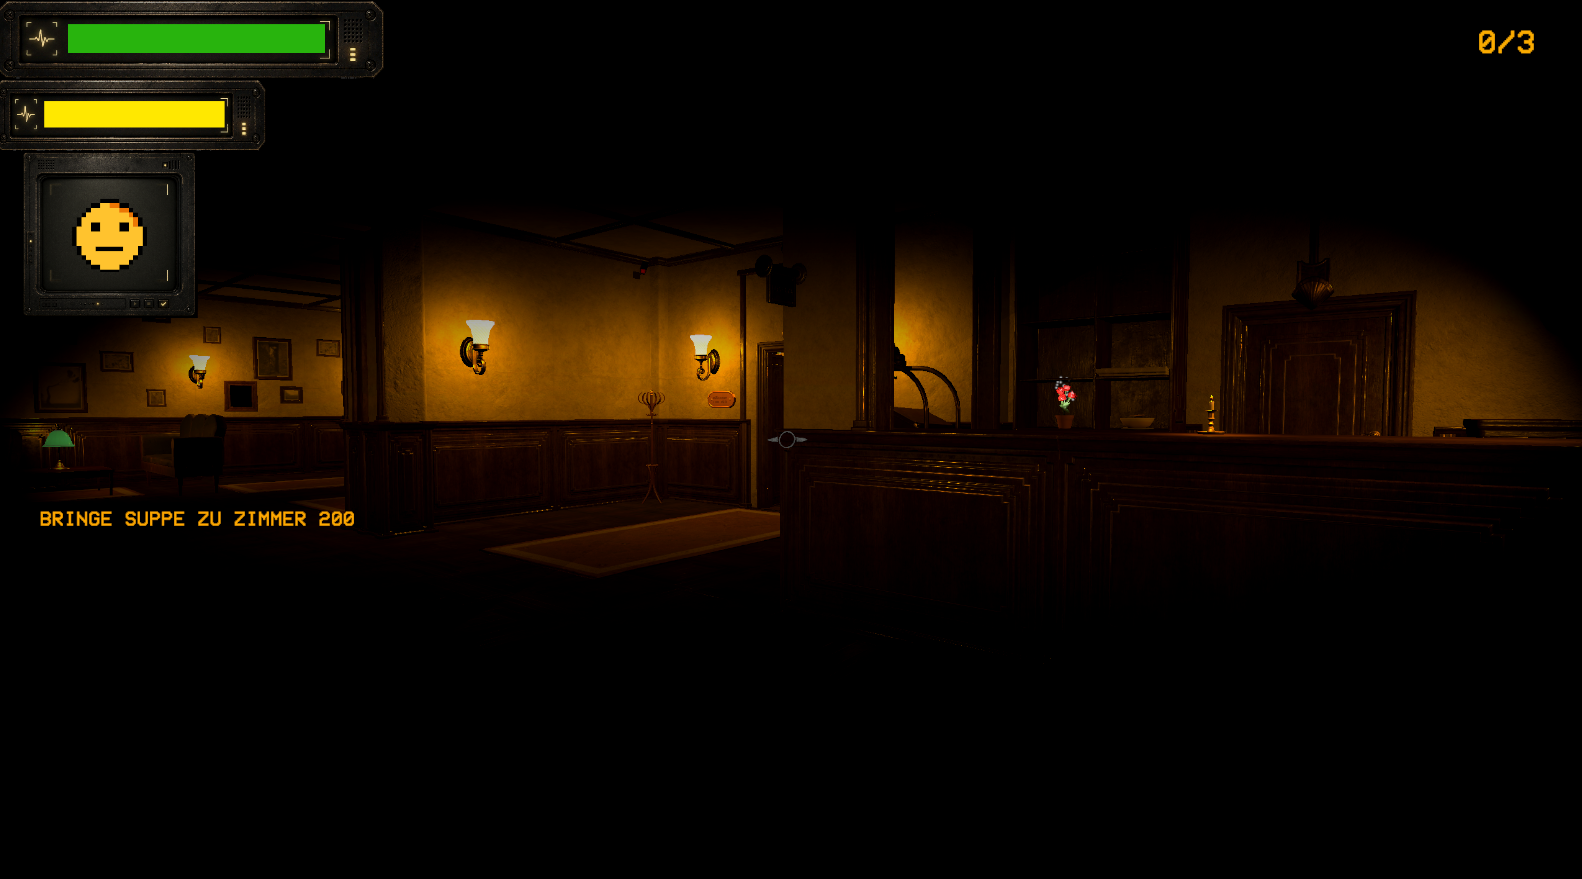
\includegraphics[width=0.8\textwidth]{Bilder/eyelidsAnimation.png}
    \caption{Screenshot aus dem Prototypen zur Darstellung der Augenlider.}
    \label{fig:facs}
\end{figure}
\subsection{Spielmodi}
Um die Wirkung der spielerbezogenen Eingaben in einer späteren Nutzerstudie (Siehe Kapitel XXX) gezielt untersuchen zu können, wurden neben dem primären, gesichtsbasierten Spielmodus (\textit{Face-Modus}) zwei weitere Spielmodi eingebaut.\\
Als zentrale Vergleichsvariante wurde ein \textit{Keyboard-Modus} entwickelt. Da der Fokus der vorliegenden Arbeit auf der Untersuchung alternativer spielerbezogener Eingaben liegt, soll dieser einen Vergleich mit einer konventionellen Eingabe über Maus und Tastatur ermöglichen. Dabei können, die sonst durch das Gesicht ausgeführten Eingaben manuell über entsprechende Tasten ausgelöst werden. Bei der Blinzelmechanik gibt es jedoch eine Besonderheit. Würde das Blinzeln ausschließlich über eine freiwillige Tasteneingabe funktionieren, bestünde für den Spieler kein Anlass zum Blinzeln. Die im Prototyp umgesetzten Mechaniken, wie der Blink-Enemy oder die Kerze, erfordern nämlich das Nicht-Blinzeln und würden somit ihre Herausforderung verlieren.\\
Aus diesem Grund wurde für diesen Modus eine Kombination aus manuellem und automatischem Blinzeln umgesetzt. Der Spieler kann selbständig über eine Taste ein Blinzeln auszulösen, gleichzeitig tritt dies jedoch auch nach einem variierenden Zeitintervall automatisch auf. Somit ist der Zeitpunkt des Blinzelns nicht immer vorhersehbar. Diese Mechanik soll die eingeschränkte Kontrollierbarkeit des menschlichen Blinzelns adaptieren und zu einer besseren Vergleichbarkeit der beiden Modis führen.\\
Ein weiterer Modus dient dazu, zu untersuchen welchen Einfluss die visuelle Darstellung des Blinzelns auf den Spieler hat. Dafür wurde hierbei die Darstellung der Augenlider ausgeschaltet. 
\section{Implementierung}
Dieses Kapitel behandelt die technische Umsetzung des in Kapitel 4 beschriebenen Konzepts des Prototypen. 
\subsection{Technische Umgebung}
Der in dieser Arbeit entwickelte Prototyp wurde mit der Game Engine Unity realisiert. Neben den klassischen Eingaben wie Maus und Tastatur erfolgt die Interaktion auch über gesichtsbasierte Daten. Dafür wird der bereits in Kapitel XXX vorgestellte MediaPipe Landmarker verwendet. Da MediaPipe nicht einfach in Unity ausgeführt werden kann, wurde die Gesichtserfassung in einem separaten Python Prozess ausgelagert. Über eine UDP-Verbindung werden die Daten anschließend an Unity übermittelt (siehe Kapitel 5.2). Durch die Implementierung verschiedener Modi wurde eine Abstraktionsebene bereitgestellt, die die Spielmechaniken unabhängig von dem Eingabemodus auf dieselben Ereignisse reagieren lässt. (sie Kapitel 4.7). 
Die von MediaPipe ausgegebenen \textit{Face Landmarks} und \textit{Blendshape Scores} stellen die Grundlage für das hier implementierte System der Blinzel- und Gesichtsausdruckserkennung dar. Der grundlegende Datenfluss der gesichtsbasierten Eingaben ist in Abbildung ~\ref{fig:systemarchitektur} dargestellt. 
\begin{figure}[H]
    \centering
    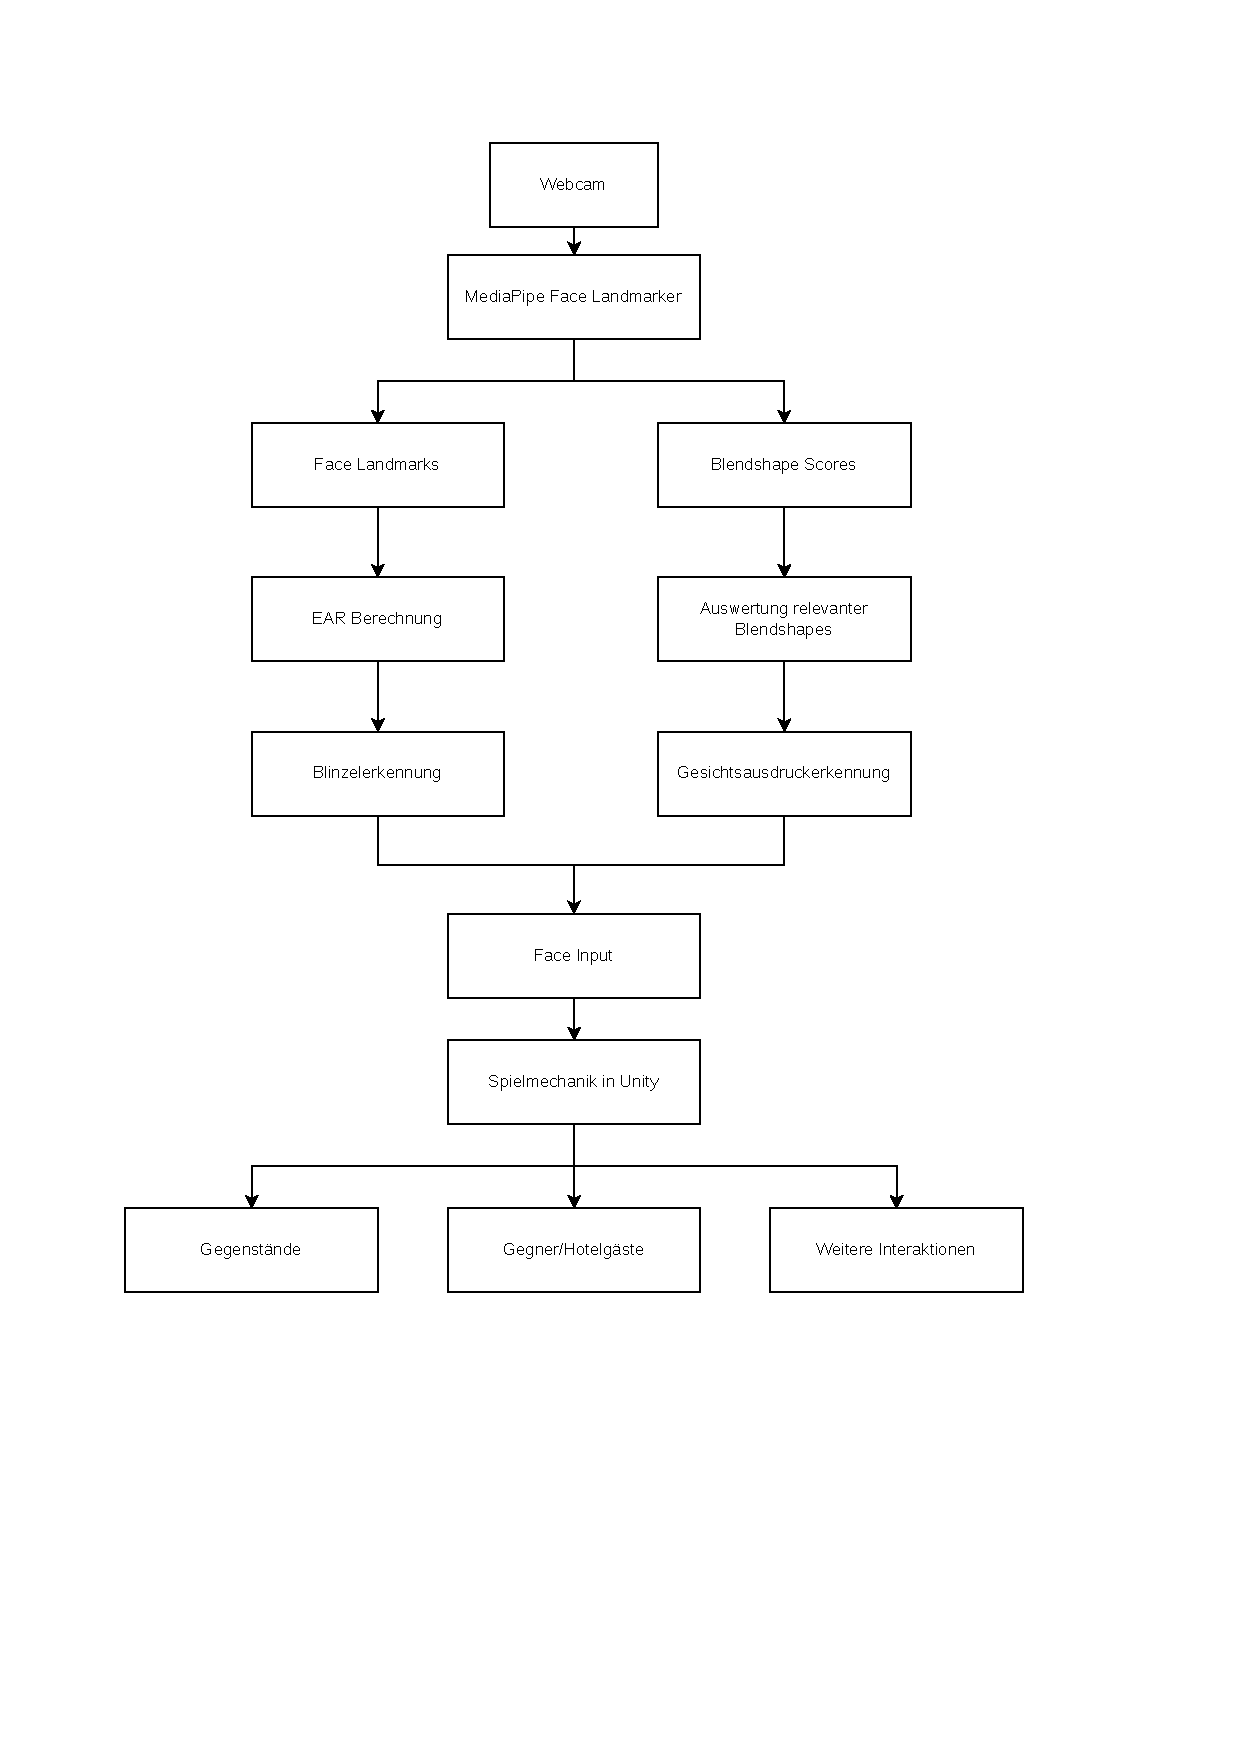
\includegraphics[width=0.9\textwidth]{SVG/systemarchitektur.pdf}
    \caption{Übersicht des Datenflusses von der Gesichtserfassung bis zur Integration in die Spielmechaniken.}
    \label{fig:systemarchitektur}
\end{figure}
Die von Mediapipe gelieferten Rohdaten werden je nach Verwendungszweck unterschiedlich weiterverarbeitet. Für die Blinzelerkennung werden hierbei die \textit{Face Landmarks} verwendet, aus denen zunächst der EAR-Wert berechnet wird. Die Erkennung der Gesichtsausdrücke basiert hingegen auf den von Mediapipe bereitgestellten \textit{Blendshape Scores}. \\
Die verarbeiteten Werte werden anschließend an die gemeinsame Klasse \textit{Face Input} weitergereicht und für die verschiedenen Spielmechaniken bereitgestellt. Diese Klasse fungiert somit als Schnittstelle zwischen der Verarbeitung der Gesichtsdaten und der darauf aufbauenden Spielmechaniken, ohne dass diese die zugrunde liegende Gesichtserkennung selbst verarbeiten müssen. \\
Neben der Verarbeitung der Gesichtsdaten besteht der Prototyp aus mehreren miteinander verbundenen Spielsystemen. Der grundlegende Spielablauf wird durch ein Delivery-System realisiert, während ein Room-System die Verwaltung der Hotelräume übernimmt. Für die Integration der Eingaben in die Spielmechaniken wird ein Condition-System verwendet. Die verschiedenen Gegnertypen basieren zudem auf einer gemeinsamen Basisklasse, die eine einheitliche Grundstruktur für ihr Verhalten bereitstellt.
Im Folgenden wird auf die einzelnen konkreten Umsetzungsschritte genauer eingegangen.
\subsection{Anbindung von MediaPipe}
Für die Anbindung von MediaPipe an Unity wurde die Gesichtserfassung in
einen separaten Python-Prozess ausgelagert. Das zugehörige Python-Programm
verarbeitet die eingehenden Kamerabilder mit dem MediaPipe Face Landmarker.
Für das erkannte Gesicht werden dabei sowohl die \textit{Face Landmarks}
als auch die \textit{Blendshape Scores} ausgelesen. Da es sich bei dem
Prototyp um ein Singleplayer-Spiel handelt und somit immer nur eine
spielende Person betrachtet wird, ist die Erkennung auf ein Gesicht
beschränkt.\\
Die erfassten Daten werden anschließend über eine lokale UDP-Verbindung
an Unity übertragen. Hierfür werden die \textit{Face Landmarks} und
\textit{Blendshape Scores} in eine JSON-Struktur überführt und über die
Loopback-Adresse \texttt{127.0.0.1} an Port \texttt{5005} gesendet.
Damit erfolgt die Kommunikation ausschließlich lokal auf dem Rechner,
auf dem der Prototyp ausgeführt wird.\\
In Unity werden die Daten von dem \texttt{UdpReceiverService}
entgegengenommen und gespeichert. Dabei werden die \textit{Face Landmarks}
in Form eines Arrays und die \textit{Blendshape Scores} in Form eines
Dictionaries abgelegt.\\
Der \texttt{MediaPipeProvider} dient anschließend als zentrale
Schnittstelle zwischen dem externen MediaPipe-Prozess und den restlichen
Systemen des Spiels. Er ist für das Starten und Stoppen des externen
Prozesses verantwortlich und stellt die empfangenen Daten für die weitere
Verarbeitung innerhalb von Unity bereit.\\
Zu Beginn der Entwicklung setzte die Ausführung des MediaPipe-Prozesses eine Installation von Python und MediaPipe auf dem Zielrechner voraus. Um diese Vorraussetzung zu vermeiden, wurde das Python-Programm mithilfe von PyInstaller in eine eigenständige ausführbare Datei überführt. Das benötigte MediaPipe-Modell
\texttt{face\_landmarker.task} wurde dabei ebenfalls in das Programmpaket
eingebunden. Die erzeugte Anwendung wird über das
\texttt{StreamingAssets}-Verzeichnis gemeinsam mit dem Spiel-Build
bereitgestellt.
Beim Start der
Gesichtserfassung wird die Anwendung über den
\texttt{PythonProcessService} als separater Prozess gestartet. Beim
Beenden der Gesichtserfassung oder der Unity-Anwendung werden sowohl
der UDP-Empfänger als auch der externe Prozess wieder beendet.
\subsection{Blinzelerkennung}
Für die Blinzelerkennung wird die bereits in
Kapitel 2.3 vorgestellte Eye Aspect Ratio (EAR) verwendet. Für die Berechnung werden die von MediaPipe bereitgestellten \textit{Landmarks} verwendet. Für das linke Auge werden hierfür die \textit{Landmarks} 33, 159,
158, 133, 153 und 145 verwendet und für das rechte Auge die \textit{Landmarks} 362, 386, 387, 263, 374 und 380. \\
Die Berechnung erfolgt in der Klasse \texttt{EARCalculator} und entspricht dabei der in Kapitel 2.3 vorgestellten Formel. Dabei wird der zunächst der EAR-Wert für beide Augen separat berechnet und daraufhin der Mittelwert gebildet. Der resultierende Wert wird für die Weiterverarbeitung der Blinzelerkennung verwendet.\\
Die Auswertung des berechneten EAR-Wertes erfolgt durch die Klasse \\ \texttt{BlinkDetector}. Dafür wird geprüft, ob der berechnete Wert unterhalb eines personenspezifischen Schwellenwertes liegt. Wie dieser Schwellenwert zustande kommt, wird später in Kapitel XXX genauer behandelt. Liegt der aktuelle EAR-Wert nun unterhalb des Schwellenwertes, dann wird dies als Beginn eines potenziellen Blinzelns wahrgenommen. Um einzelne Schwankungen nicht fälschlicherweise als Blinzeln zu registrieren, muss der EAR-Wert für mindestens zwei aufeinanderfolgende Frames unterhalb des Schwellenwertes liegen. Erst dann wird der Zustand als Beginn eines Blinzelns erkannt. Gleiches gilt für das Öffnen der Augen. Das Blinzeln gilt erst dann als beendet beziehungsweise die Augen erst dann wieder als geöffnet, wenn nachdem die Augen geschlossen waren sich der EAR-Wert für mindestens zwei aufeinanderfolgenden Frames oberhalb des Schwellenwertes befindet.\\
\subsection{Gesichtsausdruckserkennung}
Die Erkennung der Gesichtsausdrücke basiert auf den von MediaPipe
bereitgestellten \textit{Blendshape Scores}. Aufbauend auf den in
Kapitel~2.4 beschriebenen Zusammenhängen zwischen FACS Action Units
und MediaPipe-Blendshapes werden die für den Prototyp relevanten
Blendshape Scores zunächst zu AU-nahen Merkmalen zusammengefasst
\cite{turrisi2026blendshape}.\\
Die Verarbeitung der Blendshape Scores ist innerhalb der Implementierung
auf zwei zentrale Klassen aufgeteilt. Der
\texttt{EmotionFeatureCalculator} übernimmt zunächst die Aufbereitung
der von MediaPipe gelieferten Rohwerte. Hierzu werden ausgewählte
Blendshape Scores zu AU-nahen Merkmalen zusammengefasst und daraus
jeweils ein Score für die vier im Prototyp verwendeten
Gesichtsausdrücke berechnet.\\

Die anschließende Klassifikation erfolgt durch den
\texttt{EmotionDetector}. Dieser vergleicht die berechneten Scores mit
den personenspezifischen Kalibrierungswerten, prüft die jeweiligen
Schwellenwerte und berücksichtigt die zeitliche Stabilität der
Erkennung. Als Ergebnis stellt er den aktuell erkannten
Gesichtsausdruck bereit. Durch diese Aufteilung wird die Berechnung der
Gesichtsmerkmale von deren anschließender Klassifikation getrennt.\\
\begin{table}[H]
    \centering
    \caption{Zuordnung der verwendeten MediaPipe Blendshape Scores zu den AU-nahen Merkmalen.}
    \label{tab:emotion_features}
    \begin{tabular}{ll}
        \toprule
        \textbf{Merkmal} & \textbf{Verwendete MediaPipe Blendshape Scores} \\
        \midrule
        AU1  & \texttt{browInnerUp} \\
        AU2  & Mittelwert aus \texttt{browOuterUpLeft} und \texttt{browOuterUpRight} \\
        AU4  & Mittelwert aus \texttt{browDownLeft} und \texttt{browDownRight} \\
        AU5  & Mittelwert aus \texttt{eyeWideLeft} und \texttt{eyeWideRight} \\
        AU6  & Mittelwert aus \texttt{cheekSquintLeft} und \texttt{cheekSquintRight} \\
        AU7  & Mittelwert aus \texttt{eyeSquintLeft} und \texttt{eyeSquintRight} \\
        AU12 & Mittelwert aus \texttt{mouthSmileLeft} und \texttt{mouthSmileRight} \\
        AU15 & Mittelwert aus \texttt{mouthFrownLeft} und \texttt{mouthFrownRight} \\
        AU17 & \texttt{mouthShrugLower} \\
        AU23 & Mittelwert aus \texttt{mouthPressLeft} und \texttt{mouthPressRight} \\
        AU26 & \texttt{jawOpen} \\
        \bottomrule
    \end{tabular}
\end{table}
Die Auswahl der für die einzelnen Gesichtsausdrücke verwendeten
Merkmale orientiert sich an den in Kapitel~2.4 beschriebenen
AU-Kombinationen. Darüber hinaus zeigen Untersuchungen dynamischer
Gesichtsausdrücke, dass einzelne Action Units unterschiedlich stark
mit der Erkennung bestimmter Gesichtsausdrücke zusammenhängen
\cite{calvo2018kdefdyn}.\\
Auf Grundlage dieser Merkmale wird für jeden der vier im Prototyp
verwendeten Gesichtsausdrücke ein eigener Score berechnet. Die
grundsätzliche Auswahl der Merkmale orientiert sich an den zuvor
beschriebenen AU-Kombinationen. Die konkrete Gewichtung wurde dagegen
heuristisch im Verlauf der Entwicklung festgelegt. Hierfür wurde die
Erkennung wiederholt mit verschiedenen Personen erprobt und beobachtet,
welche der verwendeten Gesichtsmerkmale bei der Darstellung des
jeweiligen Ausdrucks besonders deutlich ausgeprägt waren. Merkmale,
die sich dabei als stärker ausgeprägt beziehungsweise für die
Unterscheidung als geeigneter erwiesen, erhielten einen entsprechend
größeren Einfluss auf den resultierenden Score.

Die finale Berechnung der vier Scores erfolgt wie folgt:

\begin{align}
S_{\text{Smile}} &=
0{,}7 \cdot AU12 +
0{,}3 \cdot AU6
\\[0.5em]
S_{\text{Angry}} &=
0{,}5 \cdot AU4 +
0{,}2 \cdot AU7 +
0{,}2 \cdot AU23 +
0{,}1 \cdot AU17
\\[0.5em]
S_{\text{Sad}} &=
0{,}3 \cdot AU1 +
0{,}3 \cdot AU15 +
0{,}2 \cdot AU4 +
0{,}2 \cdot AU17
\\[0.5em]
S_{\text{Surprised}} &=
0{,}4 \cdot
\left(\frac{AU1 + AU2}{2}\right)
+
0{,}4 \cdot AU26 +
0{,}2 \cdot AU5
\end{align}

Die so berechneten Scores bilden die Grundlage für die anschließende
Klassifikation. Da sich sowohl die neutrale Gesichtsmimik als auch die
Ausprägung der einzelnen Gesichtsausdrücke zwischen Personen
unterscheiden können, werden hierfür die während der
personenspezifischen Kalibrierung erfassten Neutral- und Maximalwerte
verwendet (siehe Kapitel~5.5).

Für jeden Gesichtsausdruck $e$ wird zunächst dessen aktuelle Aktivierung
als Differenz zwischen dem aktuellen Score und dem individuellen
Neutralwert bestimmt:

\begin{equation}
    A_e =
    S_{e,\text{aktuell}} -
    S_{e,\text{neutral}}
\end{equation}

Aus dem während der Kalibrierung erfassten Maximalwert wird anschließend
ein personenspezifischer Schwellenwert bestimmt:

\begin{equation}
    T_e =
    \left(
        S_{e,\text{max}} -
        S_{e,\text{neutral}}
    \right)
    \cdot f_e
\end{equation}

Ein Gesichtsausdruck wird als aktiv betrachtet, sobald seine aktuelle
Aktivierung $A_e$ den zugehörigen Schwellenwert $T_e$ überschreitet.
Für Freude und Überraschung wird ein Faktor von $0{,}5$, für Wut ein
Faktor von $0{,}4$ und für Trauer ein Faktor von $0{,}3$ verwendet.
Auch diese Faktoren wurden im Entwicklungsprozess heuristisch
festgelegt und an die bei der praktischen Erprobung beobachteten
Unterschiede zwischen den Gesichtsausdrücken angepasst.

Um kurzfristige Schwankungen der berechneten Scores nicht unmittelbar
als Wechsel des Gesichtsausdrucks zu interpretieren, wurde zusätzlich
eine zeitliche Stabilisierung umgesetzt. Für jeden Gesichtsausdruck
wird separat erfasst, über wie viele aufeinanderfolgende Frames der
jeweilige Schwellenwert überschritten wird. Erst wenn dies für
mindestens fünf aufeinanderfolgende Frames der Fall ist, wird der
Ausdruck für die Klassifikation berücksichtigt. Fällt die Aktivierung
zuvor wieder unter den Schwellenwert, wird der zugehörige Zähler
zurückgesetzt.

Da mehrere Gesichtsausdrücke gleichzeitig ihren jeweiligen
Schwellenwert überschreiten können, erfolgt abschließend eine Auswahl
zwischen allen ausreichend stabilen Ausdrücken. Hierfür wird der
Gesichtsausdruck mit der größten absoluten Aktivierung gegenüber seinem
jeweiligen Neutralwert ausgewählt. Erfüllt keiner der vier
Gesichtsausdrücke die erforderlichen Bedingungen, wird der Zustand als
neutral klassifiziert.

\subsubsection{Entwicklung der Klassifikationsmethode}

Die Gesichtsausdruckserkennung wurde während der Entwicklung mehrfach
überarbeitet. Neben der Gewichtung der zuvor beschriebenen Merkmale
wurden insbesondere die Schwellenwerte und die Auswahl des erkannten
Gesichtsausdrucks angepasst. In einer früheren Version wurde für alle
vier Gesichtsausdrücke ein einheitlicher Faktor von $0{,}4$ zur
Bestimmung des jeweiligen Schwellenwertes verwendet. Auch die
zugrunde liegende Kalibrierung unterschied sich zu diesem Zeitpunkt
noch von der finalen Umsetzung und wurde im weiteren
Entwicklungsverlauf überarbeitet (siehe Kapitel~5.5).

Im Rahmen einer informellen Vorab-Erprobung des Prototyps während eines
Studientags zeigte sich, dass die damalige Variante bei
unterschiedlichen Personen nicht ausreichend zuverlässig
funktionierte. Diese Erprobung war nicht Bestandteil der späteren
Nutzerstudie und diente nicht der systematischen Evaluation des
Prototyps, sondern der Identifikation von Problemen der
Implementierung. Dabei zeigte sich unter anderem, dass ein
einheitlicher Faktor für die verschiedenen Gesichtsausdrücke nicht
gleichermaßen geeignet war. Insbesondere bei der Erkennung von Trauer
war teilweise eine vergleichsweise starke Ausprägung des
Gesichtsausdrucks notwendig, bevor der entsprechende Schwellenwert
überschritten wurde.

Auf Grundlage dieser Beobachtungen wurden die Faktoren im weiteren
Entwicklungsverlauf expressionsspezifisch angepasst. Für Freude und
Überraschung wurde ein Faktor von $0{,}5$, für Wut von $0{,}4$ und
für Trauer von $0{,}3$ festgelegt. Die verwendeten Faktoren stellen
somit keine aus der Literatur übernommenen festen Grenzwerte dar,
sondern heuristisch bestimmte Parameter der für den Prototyp
entwickelten regelbasierten Klassifikation.

Neben der Anpassung der Schwellenwerte wurde zwischenzeitlich eine
relative Betrachtung der Emotionsaktivierung untersucht. Hierbei wurde
die aktuelle Aktivierung eines Gesichtsausdrucks in Relation zu dem
während der Kalibrierung erfassten Bereich zwischen Neutral- und
Maximalwert gesetzt:

\begin{equation}
    A_{e,\text{rel}} =
    \frac{
        S_{e,\text{aktuell}} -
        S_{e,\text{neutral}}
    }{
        S_{e,\text{max}} -
        S_{e,\text{neutral}}
    }
\end{equation}

Mit dieser Variante sollte stärker berücksichtigt werden, dass die
Ausprägung der berechneten Scores zwischen Personen und
Gesichtsausdrücken unterschiedlich sein kann. Bei der praktischen
Erprobung zeigte sich jedoch, dass eine ausschließlich relative
Betrachtung ebenfalls zu Fehlklassifikationen führen konnte. Die für
die einzelnen Gesichtsausdrücke berechneten Scores verändern sich
nicht vollständig unabhängig voneinander. Dies ist grundsätzlich auch
bei FACS-basierten Beschreibungen zu erwarten, da einzelne Action Units
Bestandteil mehrerer Gesichtsausdrücke sein können [QUELLE].

So konnte im vorliegenden System beispielsweise bei einem stark
überraschten Gesichtsausdruck gleichzeitig der für Trauer berechnete
Score ansteigen. War der während der Kalibrierung erfasste Wertebereich
für Trauer vergleichsweise klein, führte bereits eine geringe absolute
Veränderung zu einer hohen relativen Aktivierung. Dadurch konnte in
einzelnen Fällen Trauer anstelle von Überraschung klassifiziert werden.

Für die finale Umsetzung wurde daher die absolute Aktivierung gegenüber
dem personenspezifischen Neutralwert verwendet. Die individuellen
Maximalwerte werden weiterhin zur Bestimmung der personenspezifischen
Schwellenwerte berücksichtigt. Zusätzlich wurde die Klassifikation um
die zuvor beschriebene Stabilisierung über fünf aufeinanderfolgende
Frames ergänzt, um kurzfristige Schwankungen der berechneten Scores
zu reduzieren.
GRAFIK ERGÄNZEN + drüber schauen das ist nur CHATGPT
\subsection{Kalibrierung}
Änderung nach CV Tag
EAR vorher Mittelwert - jetzt Median
Cut Percentage zu hoch gewesen
Höhere Kalibrierzeit
Emotion Calibrator vorher auch anders
Threshold vorher fest auf 0.4
EmotionDetector vorher keine Kalibrierung genommen
Vorher durchschnitt genommen 
Messe Neutral werte
messe global max werte - durchschnitt von allen emotionen also eihnzeln
eine emotion wurde kalibriert und gemacht und davon wurden die durchschnitswerte genommen und dann in global max reinegschrieben.
und generell den Peak von alen werten und nicht explizit von den einzelnen emotionen
Jetzt Verfahren

\subsection{Umsetzung der Spielmechaniken}
\subsubsection{FaceInput}
\subsubsection{Gegner}
\subsubsection{Gegenstände}
\subsubsection{Umgebungs Interaktionen}
\subsubsection{Weitere Systeme}
\subsection{Spielmodi}
\section{Nutzerstudie / Evaluation}
\subsection{Hyptothesen und Versuchsdesign}
\subsection{Versuchsablauf}
\subsection{Auswertung}
Einzelne Hypothesen durchgehen
\subsection{Weitere Ergebnisse}
\section{Fazit \& Ausblick}
\newpage
\thispagestyle{empty}
\quad 
\newpage
\pagenumbering{gobble}
\printbibliography
\newpage
\thispagestyle{empty}
\quad 
\newpage
\clearpage         % oder \cleardoublepage bei zweiseitigem Druck
\listoffigures   % fuer ein eventuelles Abbildungsverzeichnis
\clearpage
\newpage
\thispagestyle{empty}
\quad 
\newpage
\end{document}